\documentclass{dependencies/acm_proc_article-sp}

\usepackage{url}
\usepackage{color}
\usepackage{verbatim}
\usepackage{listings}
\lstset{
  language=C++,             % choose the language of the code
  basicstyle=\small,       % the size of the fonts that are used for the code
  numbers=left,                   % where to put the line-numbers
  numberstyle=\footnotesize,      % the size of the fonts that are used for the line-numbers
  stepnumber=0,                   % the step between two line-numbers. If it is 1 each line will be numbered
  numbersep=5pt,                  % how far the line-numbers are from the code
  backgroundcolor=\color{white},  % choose the background color. You must add \usepackage{color}
  showspaces=false,               % show spaces adding particular underscores
  showstringspaces=false,         % underline spaces within strings
  showtabs=false,                 % show tabs within strings adding particular underscores
  %frame=single,                   % adds a frame around the code
  tabsize=2,              % sets default tabsize to 2 spaces
  captionpos=t,                   % sets the caption-position to bottom
  breaklines=false,        % sets automatic line breaking
  breakatwhitespace=false,    % sets if automatic breaks should only happen at whitespace
  escapeinside={\%}{)}          % if you want to add a comment within your code
}

% Get rid of the permission block
\makeatletter
\let\@copyrightspace\relax
\makeatother

\begin{document}

\title{ Distrivia: A Distributed Trivia Game }
\numberofauthors{3}
\author{
\alignauthor
Brian Gianforcaro \\
       \affaddr{Rochester Institute of Technology}\\
       \email{bjg1955@rit.edu}
\alignauthor
Steven Glazer \\
       \affaddr{Rochester Institute of Technology}\\
       \email{sfg6126@rit.edu}
\alignauthor
Samuel Milton \\
       \affaddr{Rochester Institute of Technology}\\
       \email{srm2997@rit.edu}
}
\maketitle

\begin{abstract}
In this paper we will discuss our decisions and detail our discoveries throughout designing a distributed trivia system, Distrivia. 
This paper will outline our motivations behind the project, the architecture, design, implementation, lessons learned, and future work for the distributed trivia system. 
The distrivia system was implemented on 3 platforms (web, Android, and iPhone) to provide multiple ways for players to stay connected. 
It also utilizes advanced distributed systems algorithms and technology such as Amazon's EC2, Riak, SSL communication, round robin DNS, and NGINX load sharing. 
All of these services provide for high availability and secure play.
\end{abstract}

\section{Project Motivation}
Our motivation for this project was to build a system that would allow people to compete across multiple platforms reliably.
High availability was a major concern for us, as it enables people to compete at all times.
This form of trivia is a multiplayer social game.
It takes advantage of a number of different platforms so that users can feel free to play on any device they prefer.
The web client ensures that almost any device will be able to connect and play.
Designing it on mobile platforms allows us to take advtange of the specific platform and lets people easily play on the go.

\section{Architecture}
\subsection{Servers}
For our servers, we are using Amazon EC2 micro instances.
These are running x86-64 Amazon Linux.
They have 8gb of network attached storage and 613mb of memory.

Each server is installed with our custom web app that services our requests.
Each one is also equipped with an instance of Riak for maintaining our database.
The Python web app utilizes the Flask web framework and we serve the application and all files with the Tornado web server, both of which are open source.
We have five servers all running our server application and hosting the databases.
Two of those are set up as hot spares in case of a failure.

Currently, we are using the NGINX \cite{nginx} in a reverse proxy configuration for our load sharing needs. This service can be used on any machine with an active internet connection and a constantly reachable IP address or DNS lookup.


\section{Design}
\begin{figure}[h!]
  \centering
    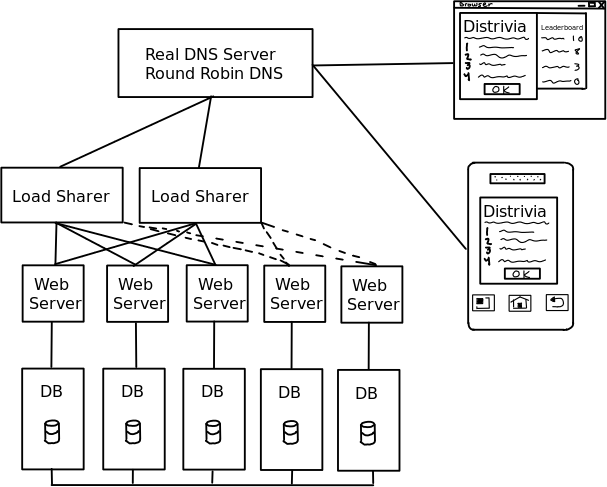
\includegraphics[scale=0.4]{diagram.png}
   \caption{High level overview of the system}
 \end{figure}
\subsection{Servers}
For this project we deployed six servers running on Amazon's Elastic Compute Cloud \cite{aec}.
One server is being used as a web-monitor host running Monit\cite{monit}.
We were able to login to the web-monitor to see the status of all our servers, databases, and load sharers.
This assisted us in managing whether or not the services were running and allowed us to track down any problems, if they arose.
Each server contains the server application that responds to clients as well as the Riak \cite{riak} databases.
Riak handles auto-synchronization of the databases between the five servers.
Note that the hot spares were setup to be part of the database cluster so they have a full copy of the database on hand, however they did not accept any reads or writes directly.
This allows for them to immediately be ready for read/writes in the event that the original servers are down.
With this configuration if we were to add a server, we would just need to update Riak and it would sync the databases to any additional servers as well.
These servers, therefore, all contain the same information.
If any servers go down, the distributed system would still run fine.
We could have all servers go down except one and still be reliably handling requests.

\subsection{Server Applications}
The server application handles requests from the user via the load sharers.
The server application supports the following features:
\begin{itemized}
\item Client registration
\item Login
\item Query games status
\item Joining public games
\item Joining private games
\item Creating private games
\item Question retrieval
\item Question answering
\item Global leaderboard
\end{itemized}

\subsection{Load Sharers}
The load sharers act as an agent between the clients and the servers to ensure reliable, fast communication.
Messages are relayed through the load sharers from the client.
Once received, the load sharer will pass the message onto any active server or, if there are none active, it will deliver the message to a hot spare server.
This is an important part of the distributed system in keeping network traffic down on the the active servers so they may serve requests faster and for making sure the server attempting to service the client's request is active and able to process the message.
They attempt to connect to a server twice in a one second period before deeming it dead and removing it from its list of servers to direct clients towards.


\subsection{Clients}
Distrivia is implemented on three distinct platforms (web, Android, and iPhone).
The clients were designed to run without specific equipment or relying on external applications. 
The clients can be run, once installed, from desktop computers, laptops, Androids, and iPhones out of box.
The web client can be run from any browser that supports CSS, which is true of all modern web browsers.
The web client can be run from any operating system that supports web browsing and has a connection to the internet (this includes mobile devices). 
This gives users of blackberry phones and palms the ability to play, even though there is not a native app for them.
The Android client will run on any Android platform running OS 2.1 or higher and does not use any unique services that require specific hardware.
Likewise, the iPhone client will run on any iPhone/iPod touch platform running any iOS without the need for specific hardware.
The Android and iPhone clients just require an active data connection either by cell signal or wireless internet.

All of our clients were designed similarly.
We tried to keep the layout as simple as possible, for the user to be able to easily navigate the game.
The mobile clients are the most similar due to their limited screen real estate.
This was important in allowing players to play on multiple platforms while using a layout they were used to.
As mobile gaming continues to grow, our approach was to promote the play of Distrivia on the go. 
Each round can be quickly played within the course of a few minutes, which makes it ideal for playing on mobile devices.
Distrivia allows users to connect with players on any other device which gives friends the opportunity to play together without forcing them to conform to one platform.

\subsection{Messages}
Distrivia uses https protocol for communication. 
This provides a secure and usable messaging system that both the client and server APIs use.
The actual messages are sent and received in two ways. 
Initially a user session key is generated using the UUID\cite{uuid} algorithm and returned to the user on successful authentication. 
This session key is then passed back to the server with every incoming
message. 
Messages are sent to the server using POST and GET request methods supported
by the HTTP protocol. 
Responses from the server are in the form of JSON \cite{json} objects.
JSON is a small, easily-parseable format, representing objects in a human readable format as they would be represented in JavaScript. 
With the web client the JSON object returned from the server is instantly usable, however for other applications, parsing the JSON object into native objects is necessary. 
% Maybe should go under implementation?
The Android SDK provides libraries to do this, located in the
org.json \cite{orgjson} package name space.
% Include the package used for iPhone and cite

\section{Implementation}
\subsection{Network}


For this project, we set up two load balancers which are running on personal desktop computers that have reliable internet connections.
The duplicate sharers allow for a load distributer to go down and we would still be able to serve requests to the servers. 
% TODO cite ZoneEdit
These are set up with round robin DNS entries, courtesy of ZoneEdit.com, a free DNS management service.
These load sharers are selected by the clients where distrivia.lame.ws will select either load distributer that is up at random. 
If a load distributer should go down or become unreachable the DNS service will no longer serve that hosts DNS record until it is again reachable.
This provides us with stability for accessing the servers.

\subsection{Clients}
% Show images of implemented clients
Creating native apps for the Android OS and iPhone gives the users the best performance on those devices along with the native look and feel of the device for optimal design.
\subsubsection{Web}

\subsubsection{Android}

\subsubsection{iPhone}

\section{Lessons Learned}

\section{Future Work}

\newpage
%
% The following two commands are all you need in the
% initial runs of your .tex file to
% produce the bibliography for the citations in your paper.
\bibliographystyle{abbrv}
\bibliography{bibliography}  % sigproc.bib is the name of the Bibliography in this case
% You must have a proper ".bib" file
%  and remember to run:
% latex bibtex latex
% to resolve all references
%
% ACM needs 'a single self-contained file'!
%
%APPENDICES are optional
\balancecolumns
% That's all folks!
\end{document}
